\documentclass[10pt,twocolumn,letterpaper]{article}

\usepackage{cvpr}
\usepackage{times}
\usepackage{epsfig}
\usepackage{graphicx,animate}
\usepackage{amsmath}
\usepackage{amssymb}

% Include other packages here, before hyperref.

% If you comment hyperref and then uncomment it, you should delete
% egpaper.aux before re-running latex.  (Or just hit 'q' on the first latex
% run, let it finish, and you should be clear).
\usepackage[pagebackref=true,breaklinks=true,letterpaper=true,colorlinks,bookmarks=false]{hyperref}

\cvprfinalcopy % *** Uncomment this line for the final submission

\def\cvprPaperID{****} % *** Enter the CVPR Paper ID here
\def\httilde{\mbox{\tt\raisebox{-.5ex}{\symbol{126}}}}

% Pages are numbered in submission mode, and unnumbered in camera-ready
\ifcvprfinal\pagestyle{empty}\fi
\begin{document}

%%%%%%%%% TITLE
\title{Brain Tumor Segmentation with Deep Neural Networks}

\author{Joshua Crowther\\
Georgia Institute of Technology\\
{\tt\small jcrowther9@gatech.edu}
\and
Lukas Dauterman\\
Georgia Institute of Technology\\
{\tt\small ldauterman3@gatech.edu}
\and
Barry Cheng\\
Georgia Institute of Technology\\
{\tt\small barrycheng@gatech.edu}
\and
Julio Moscon\\
Georgia Institute of Technology\\
{\tt\small Email@gatech.edu}
}

\maketitle
%\thispagestyle{empty}

%%%%%%%%% ABSTRACT
\begin{abstract}
    Identifying brain Tumors in MRIs is a large time cost for radiologist. This process can take days of a radiologists work, and is time critical work to identify cancer. In order to reduce the time it takes to address these issues, we are training deep neural networks on the BRATS MRIs to segment tumors in MRIs. In this we applied Unet, DeepLabV3+, and our own network. We found that our custom network performed the best on all the metrics, while Unet had the lowest false positive rate, and DeepLabV3+ had resolution issues.
\end{abstract}

%%%%%%%%% BODY TEXT
\section{Introduction}

\subsection{Problem}

Radiologists are a finite and expensive resources for identifying brain tumors in MRIs\cite{RAD}. Can we train a DNN to predict tumors in MRIs faster and more accurately than radiologists? The time saved by using a model could mean the difference between a patient living or dying.

To attempt this, we have trained 3 different models Unet, DeepLabV3+, and a custom model to identify gliomas and related tissue disorders in MRIs. 

\subsection{MRI Background}

MRIs are used to get detailed 3D image of patients brains. Radio waves stimulate radio emissions of water molecules in the brain in a strong magnetic field to generate MRIs. The pulse frequency of the radio wave results in image types base on tissue characteristics. High frequency pulses are T1 images, medium frequency are T2 images, and low frequency are FLAIR images\cite{MRI}.

Radiologists choose the MRI type depending on the cancer. The radiologist uses the MRI volume to examine slices to identify the tumors. Radiologists are a finite resource that require training and time to identify tumors\cite{RAD}.


\subsection{Data}

For training we used the BRATS 2021 dataset\cite{BRATS}. The Radiolocial Society of North America created the dataset to drive research on glioma segmentation. The MRIs were labeled by one of 4 radiologists and use the outputs of previous SOTA models. These MRIs were aligned and reshaped to match.The data set contains 1251 subject MRIs with the T1,T2,FLAIR, and segmentation images. These were saved as .nii.gz images one per image type per subject. These MRIs have had their skulls striped anonymizing the patients.

As a test set we used the IXI dataset \cite{IXI} to measure the false positive rate. This helps us calibrate model sensitivity. This data is made available by the Imperial college of London. It contains 600 T1 and T2 MRIs of health individuals. These have not been skull stripped and can potentially be used to reconstruct the patients identities. 

We ended up not using the Episurg dataset\cite{EPI} as the MRIs were not aligned for the same subject, and the labels were inconsistent shapes. This would have required software tools that we had no experience with.

%(5 points) What did you try to do? What problem did you try to solve? Articulate your objectives using absolutely no jargon. 

%(5 points) How is it done today, and what are the limits of current practice?

%(5 points) Who cares? If you are successful, what difference will it make? 

%(5 points) What data did you use? Provide details about your data, specifically choose the most important aspects of your data mentioned \href{https://arxiv.org/abs/1803.09010}{here}. You don’t have to choose all of them, just the most relevant.
%-------------------------------------------------------------------------
%------------------------------------------------------------------------
\section{Approach}

\subsection{Frameworks}


For Data-loading we used the Torchio\cite{tio} package. This package is a collection of useful functions for reading and augmenting MRIs for different tasks. We extended this by creating a methods for reading and reprocessing the BRATS dataset for training, validating, and testing the DNNs we trained. It did not have a default data loader for reading the MRIs as were provided in the kaggle dataset. It also had a built in method for downloading and loading the IXI dataset. 

For defining the data-loaders and the training methods we used Pytorch Lightning\cite{PTL} with Pytorch \cite{PT} as a general framework for defining flexible training loops. It requires that we implement our own data-loaders using their method hooks, and that we define how training is performed on each iteration. It removes the need for us to manage where the data is processed and loaded on device making it so we can focus on experiments. It also handled data logging and storing hyper-parameters of each model run. We use Pytorch to implement the models, loss functions, and metrics. We also used to implement Pixel shuffle. 

\subsection{Losses and Metrics}

To optimize the models we used Dice Loss, Log Cosh Dice Loss, and Focal Loss.Here Dise Loss \cite{SEG} is defined as  

\begin{align}
 L_{DC}(y,p) = \frac{TP(y,p)  + \epsilon}{TP(y,p)  + .5* FP(v)  + .5*FN(y,p)    + \epsilon } 
\end{align}

where TP, FP,FN are approximations of the true positive and false positive and negative rates, and $\epsilon$ is a smoothing factor. These are calculated by taking the sum of the one hot encoding of the segment mask and multiplying by the predictions such as  $TP = \text{sum}(p*y)$, $FP = \text{sum}(p*(1-y))$, and $FN = \text{sum}((1-p)*y)$. This is not directly convex and may have issues during train. To address this it has been proposed that the log cosh \cite{SEG} of the function can be used to smooth out the non convex nature of Dice Loss.

\begin{align}
L_{LC}(y,p) = \log(\cosh(L_{DC}(y,p)))
\end{align}

Another potential issue is over-fitting to the classes that have better representation in the data. For cross entropy this can be done by adjusting the equation to only learn well on examples where is is less confident called focal loss \cite{SEG}:

\begin{align}
L_{FL}(V) = \frac{1}{|V|} \sum_{v \in V}  \sum_{j = 0 }^{|C|-1} y(C_j|v) (1-p(C_j|v))^\gamma  \log(p(C_j|v) ) 
\end{align}
where $C$ is the set of class, V is the set of pixel elements in a volume, v is a pixel in V, y is the label if it is that class or not, and $C_j$ is a specific class. This has the advantage of being a convex loss function but does not directly optimize for matching the segmentation.


A problem we encountered with the losses was that $95 \% + $ of the volumes have the negative label. This was solve by assigning each class a weighting in the losses, and that the loss was calculated for each class, then found the weighted average to produce the final loss value. We also found that Jaccard and Dice Loss were very similar in formulation and could be expressed in terms of each other so we used Log Cosh loss instead as it was more interesting.

Pixel accuracy \cite{MET} can be used to measure the accuracy of the model to predict the classes for each pixel in a volume. This can be done by taking the argmax of the prediction at each pixel, checking if matches ground truth, then taking the average across the volume. 

\begin{align}
acc = \frac{1}{N |V|} \sum_{i=0}^{N-1} \sum_{v \in V} y(v|C_i) == P(v|C_I)
\end{align}

Intersection over union \cite{MET}  ca be used to tell how well  the predicted segmentation for each class intersects with ground truth. This is done as follows:

\begin{align}
mIoU = \frac{1}{N} \sum_{i=0}^{N-1} \frac{| C_i \cap P_i|}{|C_i \cup P_i|} 
\end{align}

Where $C_i$ is the set of pixel with labeled ground truth for class $i$, and $P_i$ is the model predictions for that class. Another measure of the class intersection is the Dice Coefficient \cite{MET} :

\begin{align}
dice\_coef = \frac{1}{N} \sum_{i=0}^{N-1} \frac{2| C_i \cap P_i|}{|C_i |+ | P_i|}
\end{align}

A problem we encountered was that due to the class imbalance the metrics go to $99 \%$ very quickly. We solved this by removing the negative class from the calculation so that we were only measuring  the metrics on the tumor segmentation task. This could be done because the metrics would go to 0 if the model was over fitting on the negative class.


\subsection{Models}

We did not end up using a model based on Pixel Shuffle \cite{PIX} or Depth to Space \cite{DEP}. These methods did not generalize well to 3D data, and the models always had the metrics drop to zero, meaning that back-prop was not working well for the task.


Keep it to short descriptions of Unet and DeepLabV3+ and we need to got in-depth on our custom model. 

The Deeplabv3+ model is an updated version of Deeplabv3. The architecture was improved by the authors of the original model by adding an encoder-decoder structure. The encoder is similar to DeepLabv3, but with the addition of the Separable Atrous Convolution. The Decoder consists of up-sampling operations to upscale the output of the encoder. In our Deeplabv3+ version, we replaced all 2D operations with 3d equivalent operations and for the network backbone, we implemented a 3D version of the ResNet-101.
 
The Unet model was first introduced for 2-D biomedical image segmentation tasks as an improvement upon the sliding window approach to localize and label regions around each pixel. Unet utilizes a contracting path to increase output resolution and an expanding path to combine results from the contracting path in order to localize high resolution features. 2-D Unet has provided good performance on biomedical segmentation tasks when combined with data augmentation. Our goal is to design a 3-D version of Unet to experiment if the strong segmentation performance also applies to volumes.

\subsubsection{Custom Model}

The custom model was based off of an existing 3D Unet implementation (see \cite{10.7554/eLife.57613}). Given the Unet base, many of the characteristics of the Unet model are present in the custom model as well. Unet is designed with max pooling layers in between stacks of convolutional layers. The custom model explores the effect of different aggregation and generalization with the final model using a combination of max pooling, average pooling, as well as 3D dropout layers to attempt to improve gradient flow and better propagate feature representation throughout the network.

DeepLabV3+ and Unet both have well documented architectures that can be explored in \cite{https://doi.org/10.48550/arxiv.1802.02611} and \cite{https://doi.org/10.48550/arxiv.1505.04597} respectively. The custom model used for these experiments, while taking queues from both models, is distinct from both.

In convolutional neural networks pooling is used as a down-sampling methodology that helps with overfitting while also improving computational speeds by reducing the dimensionality of the inputs. There are a number of different pooling strategies that approach the task from mathematically unique perspectives. For this effort several methods explored in \cite{https://doi.org/10.48550/arxiv.2009.07485} were considered. However, to simplify the optimization space, due to time restrictions, only max pooling and average pooling were used.

As with Unet, the custom model uses stacks of convolutional layers as encoding layers each separated by pooling layers. Each encoding stack increasing the channel depth of the previous input. The first two encoding layers use max pooling, while the second two use average pooling. The architecture can be seen in figure \ref{fig:custom-model-arch}.

\begin{figure}[h]
\centering
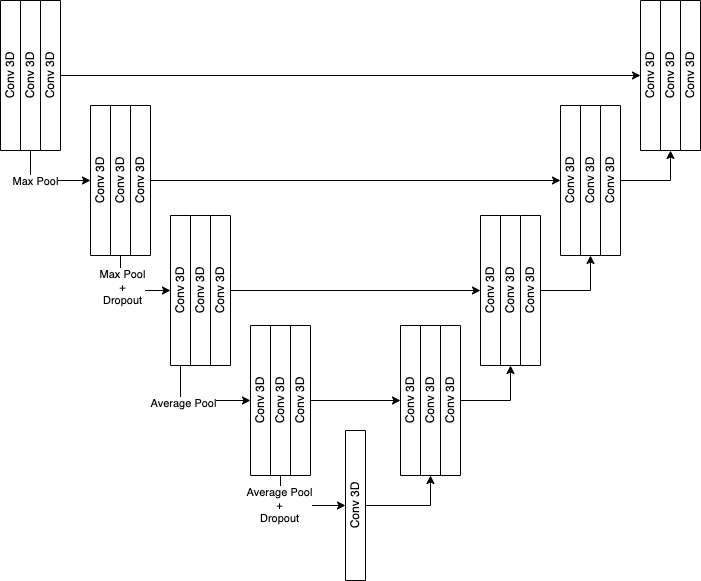
\includegraphics[width=0.5\textwidth]{figures/custom-model.png}
\caption{Custom network model architecture}
\label{fig:custom-model-arch}
\end{figure}
\subsection{Methodology}

Do we want to go in-depth on methodology here?


(10 points) What did you do exactly? How did you solve the problem? Why did you think it would be successful? Is anything new in your approach? 

(5 points) What problems did you anticipate? What problems did you encounter? Did the very first thing you tried work? 

\textbf{Important: Mention any code repositories (with citations) or other sources that you used, and specifically what changes you made to them for your project. }

\section{Experiments and Results}

(10 points) How did you measure success? What experiments were used? What were the results, both quantitative and qualitative? Did you succeed? Did you fail? Why? Justify your reasons with arguments supported by evidence and data.

\textbf{Important: This section should be rigorous and thorough. Present detailed information about decision you made, why you made them, and any evidence/experimentation to back them up. This is especially true if you leveraged existing architectures, pre-trained models, and code (i.e. do not just show results of fine-tuning a pre-trained model without any analysis, claims/evidence, and conclusions, as that tends to not make a strong project). }

%-------------------------------------------------------------------------
\section{Other Sections}

\begin{table*}
\begin{center}
\begin{tabular}{|l|c|p{8cm}|}
\hline
\centering \textbf{Student Name} & \textbf{Contributed Aspects} & \textbf{Details} \\\hline

Lukas Dauterman & Identified Data-sets & Did the work to identify and Collect datasets appropriate for use in the project \\\hline
Lukas Dauterman & Data Loading & Implemented the method for loading using Torchio and reprocessing the BRATS Data-set \\\hline
Lukas Dauterman & Training Methods & Created Framework for running experiments in  PyTorch lighting, fully integrating the data-loaders, models, and metrics and prepossessing pipeline \\\hline
Lukas Dauterman & Losses and Metrics & Wrote from scratch the loss functions and metrics, and adjusted them once the class imbalanced issue was identified. \\\hline
Lukas Dauterman & Implemented Pixel Shuffle and Model & Wrote a 3D Implementation of Pixel shuffle due to Pytorch not supporting 3D, and wrote model using Pixel Shuffle base don Unet \\\hline

Josh Crowther & Collaboration Setup & Integrated workflow tooling to facilitate collaboration between members of the team \\\hline
Josh Crowther & Platform standardization & Consolidated the various training implementations that were being used for reproducible training and validation \\\hline
Josh Crowther & Experiment Scripting & Gathered requirements on hyperparameter tuning, authored, and validated scripts used for running all model experiments \\\hline
Josh Crowther & Custom Model Design/Implementation & Researched the strategy for diverse aggregation methods and implemented the custom model based on that research \\\hline

Julio Moscon & CATEGORY OF THING & DESCRIPTION OF THE THING \\\hline

Barry Cheng & CATEGORY OF THING & DESCRIPTION OF THE THING \\\hline

\end{tabular}
\end{center}
\caption{Contributions of team members.}
\label{tab:contributions}
\end{table*}

You are welcome to introduce additional sections or subsections, if required, to address the following questions in detail. 

(5 points) Appropriate use of figures / tables / visualizations. Are the ideas presented with appropriate illustration? Are the results presented clearly; are the important differences illustrated? 

(5 points) Overall clarity. Is the manuscript self-contained? Can a peer who has also taken Deep Learning understand all of the points addressed above? Is sufficient detail provided? 

(5 points) Finally, points will be distributed based on your understanding of how your project relates to Deep Learning. Here are some questions to think about: 

What was the structure of your problem? How did the structure of your model reflect the structure of your problem? 

What parts of your model had learned parameters (e.g., convolution layers) and what parts did not (e.g., post-processing classifier probabilities into decisions)? 

What representations of input and output did the neural network expect? How was the data pre/post-processed?
What was the loss function? 

Did the model overfit? How well did the approach generalize? 

What hyperparameters did the model have? How were they chosen? How did they affect performance? What optimizer was used? 

What Deep Learning framework did you use? 

What existing code or models did you start with and what did those starting points provide? 

Briefly discuss potential future work that the research community could focus on to make improvements in the direction of your project's topic.

%-------------------------------------------------------------------------

{\small
\bibliographystyle{ieee_fullname}
\bibliography{egbib}
}

\end{document}
